\section{Síntesis de voz neuronal}

La síntesis de voz, o \textit{text-to-speech} (TTS), consiste en transformar una secuencia de texto en una señal de audio inteligible y natural. En sistemas modernos, esta tarea se aborda mediante modelos neuronales capaces de aprender la relación entre el contenido lingüístico de entrada y las características acústicas de la voz generada.

\subsection{Evolución de los modelos neuronales de voz}

La síntesis de voz neuronal ha evolucionado desde sistemas secuenciales como Tacotron 2 \citep{shen2018tacotron}, que convierte texto en espectrogramas, combinados con vocoders neuronales como WaveNet \citep{oord2016wavenet} o HiFi-GAN \citep{kong2020hifigan}, hacia modelos más flexibles capaces de clonación de voz, generación multilingüe y cierto control prosódico, es decir, control sobre aspectos como la entonación, el ritmo, las pausas o el énfasis de la voz generada.


\subsection{Síntesis multilingüe con XTTS}

XTTS \citep{casanova2024xtts} es un modelo de síntesis multilingüe \textit{zero-shot} que permite generar voz a partir de una pequeña referencia de audio y producir habla en distintos idiomas. Esta clase de modelos resulta útil cuando se desea obtener una voz concreta sin entrenar un modelo desde cero para cada locutor.

La \hyperref[fig:xtts-arquitectura]{Figura~\ref*{fig:xtts-arquitectura}} resume de forma simplificada el flujo general de XTTS. El bloque 1 corresponde al audio de referencia del hablante, a partir del cual se extrae una representación de voz. El bloque 2 representa el texto de entrada, que se tokeniza y se introduce en el modelo autoregresivo. El bloque 3 corresponde al codificador basado en GPT-2, encargado de predecir códigos discretos de audio condicionados por el texto y por la voz de referencia. Durante el entrenamiento, el bloque 4 proporciona el objetivo acústico a partir del espectrograma real. Finalmente, el bloque 5 corresponde al vocoder, que transforma los códigos generados en la onda de audio final.


\begin{figure}[H]
    \centering
    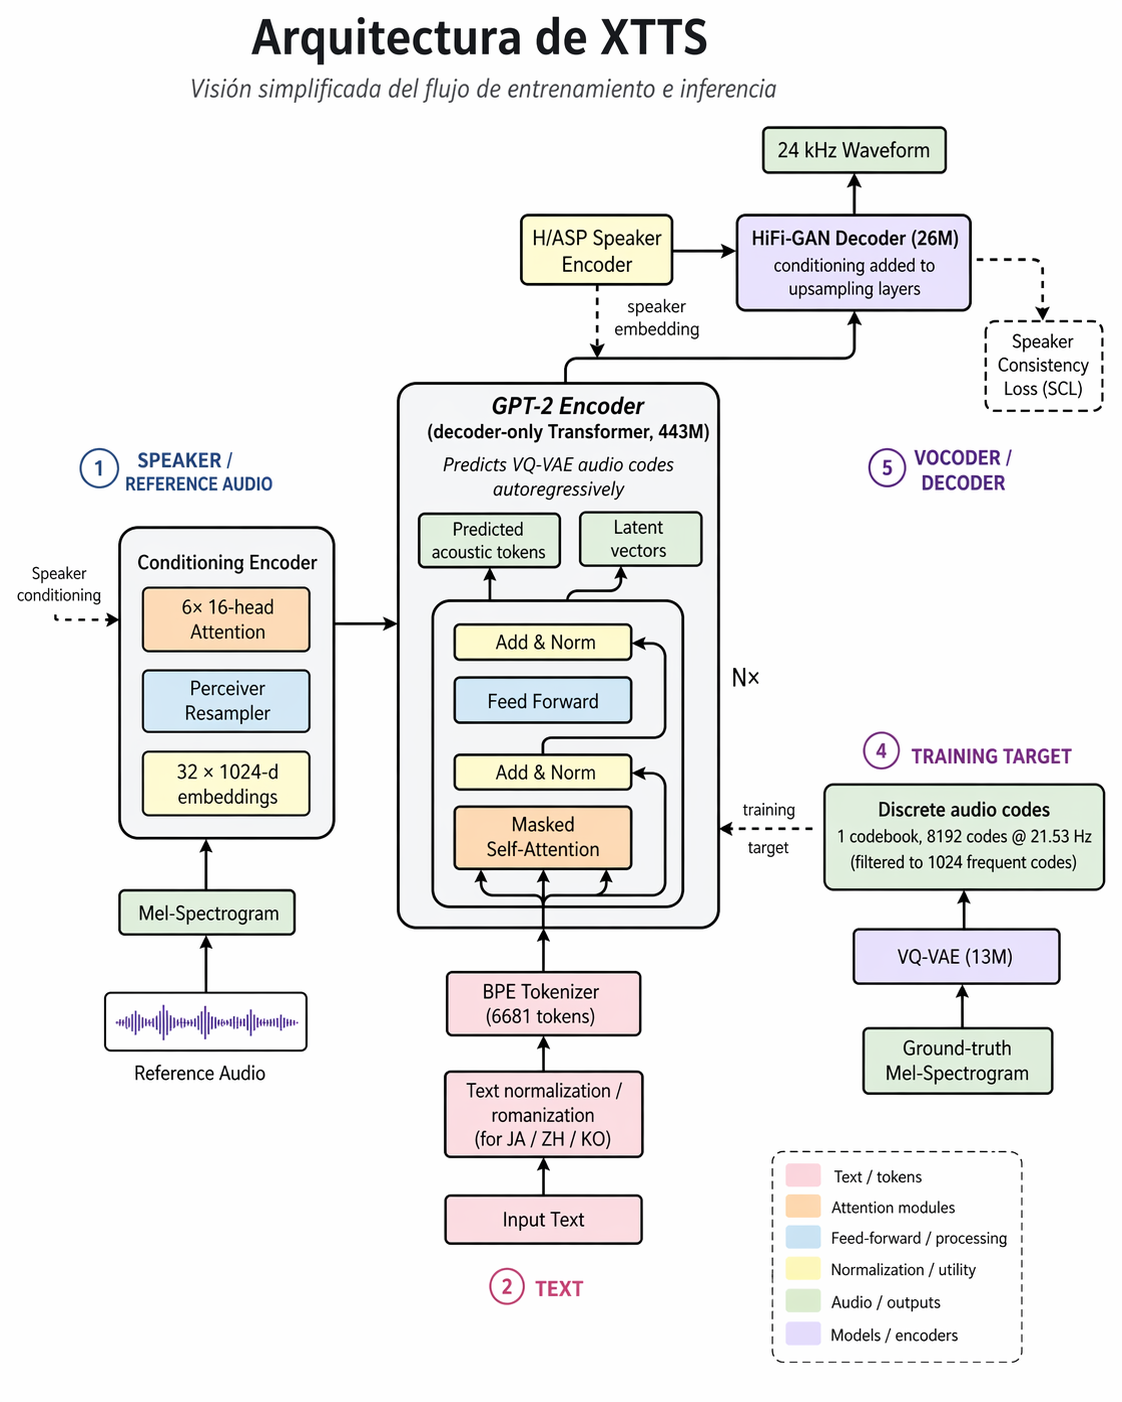
\includegraphics[width=0.9\textwidth]{Imagenes/Propias/Xtts.png}
    \caption[Diagrama general del flujo de XTTS]{
    Diagrama general del flujo de XTTS a partir de texto de entrada y audio de referencia. Fuente: elaboración propia asistida por GPT-Images-2.0 de OpenAI.
    }
    \label{fig:xtts-arquitectura}
\end{figure}

Esta arquitectura permite generar una voz condicionada por una referencia corta de audio, manteniendo cierta identidad del hablante sin necesidad de entrenar un modelo específico desde cero para cada comentarista.

\subsection{Papel de la síntesis de voz dentro del pipeline}

En el contexto de este proyecto, la síntesis de voz transforma los comentarios generados por el modelo de lenguaje en una narración audible. Esta fase cierra el flujo del sistema, convirtiendo eventos detectados y comentarios textuales en audio sincronizable con el vídeo.

En una tarea de narración deportiva, no basta con que la voz generada sea inteligible. También resultan importantes la latencia, la expresividad, la naturalidad en español y la capacidad de mantener un estilo consistente. Por este motivo, el módulo de TTS debe producir audio con suficiente calidad, pero también con un coste temporal asumible dentro del pipeline.

La implementación concreta del módulo de síntesis de voz se describe posteriormente en la \hyperref[sec:sintesis-voz-pipeline]{Sección~\ref*{sec:sintesis-voz-pipeline}}.
